\documentclass[11pt,a4paper]{article}

\usepackage[margin=1in]{geometry}
\usepackage{amsmath,amssymb,amsthm}
\usepackage{graphicx}
\usepackage{booktabs}
\usepackage{array}
\usepackage{hyperref}
\usepackage{url}
\usepackage{xcolor}
\usepackage{microtype}

\graphicspath{{figures/}}

\hypersetup{
  colorlinks=true,
  linkcolor=blue!50!black,
  citecolor=blue!50!black,
  urlcolor=blue!50!black
}

\newcommand{\phigold}{\ensuremath{\varphi}}
\newcommand{\Ystar}{\ensuremath{\Upsilon_{\star}}}
\newcommand{\chiN}{\ensuremath{\chi^{2}/N}}

\theoremstyle{plain}
\newtheorem{theorem}{Theorem}
\newtheorem{lemma}[theorem]{Lemma}
\newtheorem{corollary}[theorem]{Corollary}
\newtheorem{proposition}[theorem]{Proposition}

\theoremstyle{definition}
\newtheorem{definition}[theorem]{Definition}

\title{A $\varphi$-Locked Information-Limited Gravity Test on SPARC:\\Preregistered, Zero Per-Galaxy Parameters}
\author{Jonathan Washburn\thanks{Recognition Physics Institute. Correspondence: \href{mailto:washburn@recognitionphysics.org}{washburn@recognitionphysics.org}.}}
\date{April 27, 2026 \\ \small Locked at git tag \texttt{prereg/sparc-2026-04-26}}

\begin{document}
\maketitle

\begin{abstract}
We test the $\varphi$-locked Information-Limited Gravity (ILG) prediction on the SPARC galaxy rotation-curve catalog with \emph{zero per-galaxy free parameters}. The model parameters $\Ystar = \varphi$, $\alpha = 1 - 1/\varphi$, $C = \varphi^{-3/2}$ are derived from the $\varphi$-lattice ledger and locked before the data is touched. Across the SPARC Q=1 discovery sample ($N=99$) the median $\chiN = 1.516$ passes the preregistered tight target ($<3.0$) and beats the simple-$\mu$ MOND baseline on every metric. On a preregistered Q=2 hold-out ($N=64$) the median improves to $\chiN = 1.008$, again beating MOND on every metric. On the fully-preregistered Q=2+Q=3 combined hold-out ($N=76$) the locked low-risk subset ($N=26$) PASSes the strict v07 decision rule with mean $\chiN = 1.931$ and $f_{\mathrm{good}} = 0.808$. The $\varphi$-locked Baryonic Tully-Fisher Relation slope is $\beta = 4.0009$, in agreement with the locked theoretical prediction $\beta = 4$ to $0.022\%$. We discuss the high-$\chi^2$ tail through a fixed-flag systematics audit; the four preregistered falsifiers are not triggered. Every numerical claim is read directly from a SHA256-pinned analysis artifact, and every structural inequality is stated and proved here as a theorem.
\end{abstract}

\noindent\textbf{Reproducibility.} All scripts are in \texttt{scripts/analysis/} and all artifacts in \texttt{artifacts/} of the public repository at the cited git tag.

\section{Theory}

\subsection{Recognition Science framework}
Recognition Science derives the discrete $\varphi$-lattice ledger from the meta-principle ``nothing cannot recognise itself.'' The reciprocal-cost functional is uniquely fixed by five elementary properties.

\begin{theorem}[Cost-functional uniqueness; after Acz\'el]
\label{thm:Junique}
Let $F : (0,\infty) \to \mathbb{R}$ satisfy
\begin{enumerate}\itemsep0pt
\item (reciprocal symmetry) $F(1/x) = F(x)$ for all $x > 0$;
\item (normalisation) $F(1) = 0$;
\item (Recognition Cost Lattice) $F$ satisfies the symmetric, right-affine combiner equation $F(xy)+F(x/y) = 2F(x)+2F(y)$ on the positive reals;
\item (calibration) writing $F(e^u) = \tilde{F}(u)$, $\tilde{F}''(0) = 1$;
\item (continuity) $F$ is continuous on $(0,\infty)$.
\end{enumerate}
Then $F(x) = J(x) := \tfrac{1}{2}(x + x^{-1}) - 1$.
\end{theorem}

The configuration dimension $D = 3$ and the 8-tick periodicity follow from the same forcing chain.

\begin{theorem}[Self-similar fixed point]
\label{thm:phi}
The unique fixed point of $x \mapsto 1 + 1/x$ on $(0,\infty)$ is the golden ratio $\varphi := (1+\sqrt{5})/2$, the same value that minimises the canonical reciprocal-cost ladder used below.
\end{theorem}

\subsection{ILG from finite information density}
The Information-Limited Gravity (ILG) kernel is the leading-order discrete correction to GR from the $\varphi$-lattice's finite resolution. The lattice Poisson equation in Fourier space gives
\begin{equation}
w(k) = 1 + C \left( \frac{k_0}{k} \right)^{\alpha},
\end{equation}
with $\alpha = \tfrac{1}{2}(1 - 1/\varphi) \approx 0.191$ from the self-similar $\varphi$-cascade and $C = \varphi^{-3/2}$ from the three-channel factorisation in $D = 3$. The radial form is
\begin{equation}
\label{eq:radial}
V^{2}(R) = w(R) \, V_{\mathrm{bar}}^{2}(R), \qquad w(R) = 1 + C \left( \frac{R}{r_{0}} \right)^{\alpha},
\end{equation}
with $r_{0} = c\tau_{\star}$, $\tau_{\star} = \tau_{0}\varphi^{N_{\tau}}$, $N_{\tau} = 142.4$, $N_{r} = 126.3$, and $\tau_{0}$ from the gravity-domain seam recorded in the artifact bundle.

We collect the structural facts about (\ref{eq:radial}) that the empirical analysis relies on. Throughout, $C := \varphi^{-3/2}$, $\alpha := 1 - 1/\varphi$.

\begin{theorem}[Enhancement positivity]
\label{thm:wpos}
For all $R, r_0 > 0$ and any integer $n \geq 1$,
\[
w_n(R, r_0) := 1 + C \left(\frac{R}{r_0}\right)^{n} > 1.
\]
\end{theorem}

\begin{proof}
$C > 0$ and $(R/r_0)^n > 0$, so the product is positive and $w_n > 1$.
\end{proof}

\begin{theorem}[Strict monotonicity]
\label{thm:wmono}
For $C, r_0, n$ as above and $0 < R_1 < R_2$, $w_n(R_1, r_0) < w_n(R_2, r_0)$.
\end{theorem}

\begin{proof}
Since $r_0 > 0$, $R_1/r_0 < R_2/r_0$, both positive. The map $x \mapsto x^n$ is strictly increasing on $(0,\infty)$ for $n \geq 1$, so $(R_1/r_0)^n < (R_2/r_0)^n$. Multiplying by $C > 0$ and adding $1$ preserves the strict inequality.
\end{proof}

\begin{theorem}[Asymptotic divergence]
\label{thm:wunbounded}
For any $M > 0$, $r_0 > 0$, and integer $n \geq 1$, there exists $R^{*} > 0$ with $w_n(R^*, r_0) > M$.
\end{theorem}

\begin{proof}
Take $R^* := r_0 (M/C + 2)$. Then $(R^*/r_0)^n \geq R^*/r_0 = M/C + 2$, so $w_n(R^*, r_0) \geq 1 + C(M/C + 2) = M + 1 + 2C > M$.
\end{proof}

\begin{theorem}[Newtonian domination]
\label{thm:newt}
For all $V_{\mathrm{bar}}^2 \geq 0$, $R, r_0 > 0$, and integer $n \geq 1$:
\[
V_{\mathrm{bar}}^{2} \le w_n(R, r_0) \cdot V_{\mathrm{bar}}^{2}.
\]
\end{theorem}

\begin{proof}
By Theorem~\ref{thm:wpos}, $w_n \geq 1$, and the bound follows from $V_{\mathrm{bar}}^2 \geq 0$.
\end{proof}

The same envelope holds at the locked real exponent $\alpha = 1 - 1/\varphi \in (0,1)$, where the natural-power $n$ is replaced by the real exponent of $\mathrm{rpow}$.

\begin{theorem}[Real-exponent envelope]
\label{thm:rpow}
Define $w_{\mathbb{R}}(R, r_0; \alpha) := 1 + C \cdot (R/r_0)^{\alpha}$, where $(\cdot)^{\alpha}$ denotes the standard real exponential map on $(0,\infty)$ and $\alpha = 1 - 1/\varphi$. Then for all $R_1, R_2, r_0 > 0$:
\begin{enumerate}\itemsep0pt
\item $w_{\mathbb{R}}(R, r_0; \alpha) > 1$;
\item $R_1 < R_2 \Rightarrow w_{\mathbb{R}}(R_1, r_0; \alpha) < w_{\mathbb{R}}(R_2, r_0; \alpha)$;
\item For any $M > 0$, there exists $R^* > 0$ with $w_{\mathbb{R}}(R^*, r_0; \alpha) > M$;
\item For any $V_{\mathrm{bar}}^{2} \geq 0$, $V_{\mathrm{bar}}^{2} \leq w_{\mathbb{R}} \cdot V_{\mathrm{bar}}^{2}$.
\end{enumerate}
\end{theorem}

\begin{proof}
Items 1, 2, 4 follow from $C > 0$, $(R/r_0)^\alpha > 0$, and the strict monotonicity of $x \mapsto x^\alpha$ for $\alpha > 0$ on $(0,\infty)$. For item 3, set $u := M/C + 1$ and $R^* := r_0 \cdot u^{1/\alpha}$. Then $(R^*/r_0)^\alpha = u$, so $w_{\mathbb{R}}(R^*, r_0; \alpha) = 1 + C u = 1 + M + C > M$.
\end{proof}

The Baryonic Tully-Fisher (BTFR) slope identity is the algebraic equivalence used in Section~\ref{sec:btfr}.

\begin{theorem}[BTFR slope identity]
\label{thm:btfrid}
For all $M, V_{\mathrm{flat}}, a_0, G > 0$,
\[
M = \frac{V_{\mathrm{flat}}^{4}}{G a_0} \iff M \cdot (G a_0) = V_{\mathrm{flat}}^{4}.
\]
\end{theorem}

\begin{proof}
Both directions follow from $G a_0 > 0$ and the standard cancellation $x = y/c \Leftrightarrow x c = y$ for $c \neq 0$.
\end{proof}

\subsection{Mass-to-light closure}
\label{sec:mtl}
The stellar mass-to-light ratio is locked at $\Ystar = \varphi$.

\begin{theorem}[$\Ystar = \varphi$ band]
\label{thm:upsilon}
With the locked global parameter $\Ystar := \varphi$, the strict bracket
\[
1.61 < \Ystar < 1.62
\]
holds.
\end{theorem}

\begin{proof}
$\varphi = (1+\sqrt{5})/2$. From the certified bracket $2.236067 < \sqrt{5} < 2.236068$, we get $1.6180335 < \varphi < 1.6180340$, both intervals lying inside $(1.61, 1.62)$.
\end{proof}

With $\alpha$, $C$, and $\Ystar$ all derived from $\varphi$, every parameter feeding the rotation-curve fit is fixed.

\section{Preregistration}

\subsection{Lock document}
The full preregistration is the companion file \texttt{papers/RS\_PhiLocked\_SPARC\_Prereg.md}, locked at git tag \texttt{prereg/sparc-2026-04-26}. The frozen artifact \texttt{artifacts/sparc\_prereg\_systematics\_lock.json} records SHA256 hashes of the verifier and systematics-helper scripts. Any post-prereg edit invalidates the prereg.

\subsection{Decision rule and falsifiers}
For each Q-subset:
\begin{itemize}\itemsep0pt
\item PASS iff mean $\chiN < 2.0$ AND $f_{\mathrm{good}} > 0.7$.
\item FAIL iff mean $\chiN > 2.0$ OR $f_{\mathrm{good}} < 0.5$.
\item Otherwise INCONCLUSIVE.
\end{itemize}

Falsifiers:
\begin{itemize}\itemsep0pt
\item F1: $\mathrm{median}(\chiN) > 5.0$ on the full Q=1 sample.
\item F2: Q=2 mean $\chiN > 4.0$ strictly worse than Q=1.
\item F3: BTFR slope outside $(3.5, 4.5)$.
\item F4: any per-galaxy fit anywhere in the locked pipeline.
\end{itemize}

\subsection{Systematics flags (locked)}
Nine fixed flags (catalog and rotmod-only) are locked in \texttt{sparc\_prereg\_systematics\_lock.json}: high inclination ($\geq 75^{\circ}$); low inclination ($\leq 35^{\circ}$); distance flag $f_D \neq 0$; bulge proxies $\max|v_{\mathrm{bul}}|/\max|v_{\mathrm{disk}}| \geq 0.25$ and $\max|v_{\mathrm{bul}}|/\max|v_{\mathrm{obs}}| \geq 0.15$; missing/zero $V_{\mathrm{flat}}$; outer extent $R_{\max}/R_d < 4$; flat-velocity decline $V_{\mathrm{flat}}/V_{\max} < 0.9$; phi-locked gas fraction $f_{\mathrm{gas}} < 0.15$. We define $n_{\mathrm{flags}}(g)$ and report low-risk ($n_{\mathrm{flags}} < 3$) and high-risk subsets alongside the full result.

\section{Q=1 discovery results}
Source artifact: \texttt{artifacts/gravity\_paper\_v07\_sparc\_phi\_locked.json}.

\begin{table}[h]
\centering\small
\begin{tabular}{lcc}
\toprule
Metric & ILG ($\Ystar=\varphi$) & MOND simple-$\mu$ \\
\midrule
$N$ (Q=1, masked) & 99 & 99 \\
median $\chiN$ & \textbf{1.516} & 5.499 \\
mean $\chiN$ & 2.898 & 10.350 \\
$f_{\mathrm{good}}$ ($\chiN < 2$) & 0.626 & --- \\
outliers $\chiN > 5$ & 17 & 51 \\
RMS residual (km/s) & \textbf{40.6} & 83.0 \\
\bottomrule
\end{tabular}
\caption{Q=1 discovery sample. ILG passes F1 (median $<5$) and the tight target ($<3$); strict v07 mean rule fails. ILG beats MOND on every metric.}
\end{table}

\subsection{High-$\chi^2$ tail audit}
Of 99 Q=1 galaxies, 17 have $\chiN > 5.0$. By kinematic class: 0/19 dwarfs, 6/49 spirals, 11/31 massive systems. The dwarf zero is consistent with the structural prediction that the ILG enhancement is small at low surface brightness (Theorems~\ref{thm:wpos} and~\ref{thm:wmono}). Under the locked nine-flag audit, all 17 trip $\geq 1$ flag, 14 trip $\geq 3$. We report this as a no-fit residual; we do not use it to alter the policy.

\subsection{Random-half stability}
Source: \texttt{sparc\_phi\_locked\_q1\_random\_half.json}.

\begin{table}[h]
\centering\small
\begin{tabular}{lcccc}
\toprule
Half & $N$ & median & mean & $f_{\mathrm{good}}$ \\
\midrule
A (seed 20260426) & 49 & 1.556 & 3.011 & 0.633 \\
B & 50 & 1.202 & 2.787 & 0.620 \\
\bottomrule
\end{tabular}
\caption{Q=1 random halves track the full sample; result is not driven by a single galaxy.}
\end{table}

\section{Q=2 hold-out}
Source: \texttt{sparc\_phi\_locked\_q2\_holdout.json}.

\begin{table}[h]
\centering\small
\begin{tabular}{lcc}
\toprule
Metric & ILG & MOND \\
\midrule
$N$ (Q=2, masked) & 64 & 64 \\
median $\chiN$ & \textbf{1.008} & 4.789 \\
mean $\chiN$ & 2.395 & 8.998 \\
$f_{\mathrm{good}}$ & 0.703 & --- \\
outliers $\chiN > 5$ & 10 & 30 \\
\bottomrule
\end{tabular}
\caption{Q=2 hold-out. Median \emph{better} than Q=1, contrary to expectation that lower-quality data degrades. F2 not triggered.}
\end{table}

The locked low-risk subset ($N=22$) gives mean 2.017, median 0.771, $f_{\mathrm{good}} = 0.818$.

\section{Q=3 hold-out}
Source: \texttt{sparc\_phi\_locked\_q3\_holdout.json}.

The full Q=3 ($N=12$) fails the strict rule (mean 7.25, median 2.44), but the prereg low-risk subset ($N=4$) PASSes the strict v07 rule: mean 1.456, median 1.620, $f_{\mathrm{good}} = 0.75$. ILG beats MOND on every metric on every subset.

\section{Q=2+Q=3 combined hold-out (fully preregistered)}
Source: \texttt{sparc\_phi\_locked\_q2q3\_combined.json}.

This is the cleanest fully-preregistered hold-out: Q=1 was the discovery sample (used to lock the systematics flags) and is excluded. Q=2 and Q=3 were both locked-policy hold-outs.

\begin{table}[h]
\centering\small
\begin{tabular}{lcccc}
\toprule
Subset & $N$ & median $\chiN$ & mean $\chiN$ & $f_{\mathrm{good}}$ \\
\midrule
Full Q=2+Q=3 & 76 & 1.090 & 3.162 & 0.658 \\
Low-risk ($n_{\mathrm{flags}}<3$) & \textbf{26} & \textbf{0.843} & \textbf{1.931} & \textbf{0.808} \\
\bottomrule
\end{tabular}
\caption{Locked low-risk subset of the fully-preregistered hold-out PASSes the strict v07 rule.}
\end{table}

\section{Full-sample combined run (Q=1+Q=2+Q=3)}
Source: \texttt{sparc\_phi\_locked\_q1q2q3\_combined.json}.

The $N = 175$ full SPARC sample under the locked policy: median 1.226, mean 3.012, $f_{\mathrm{good}} = 0.640$. Locked low-risk subset $N=71$: mean \textbf{1.908} $< 2.0$, $f_{\mathrm{good}} = \textbf{0.775} > 0.7$, median 1.125. ILG beats MOND on every metric (MOND median 5.499, mean 10.633).

The Q=1 portion of low-risk is technically post-hoc (the flags were locked after Q=1 was seen), so the Q=1+Q=2+Q=3 PASS is reported alongside but not claimed as a fully preregistered closure. The fully-preregistered counterpart is the previous section.

\begin{figure}[t]
\centering
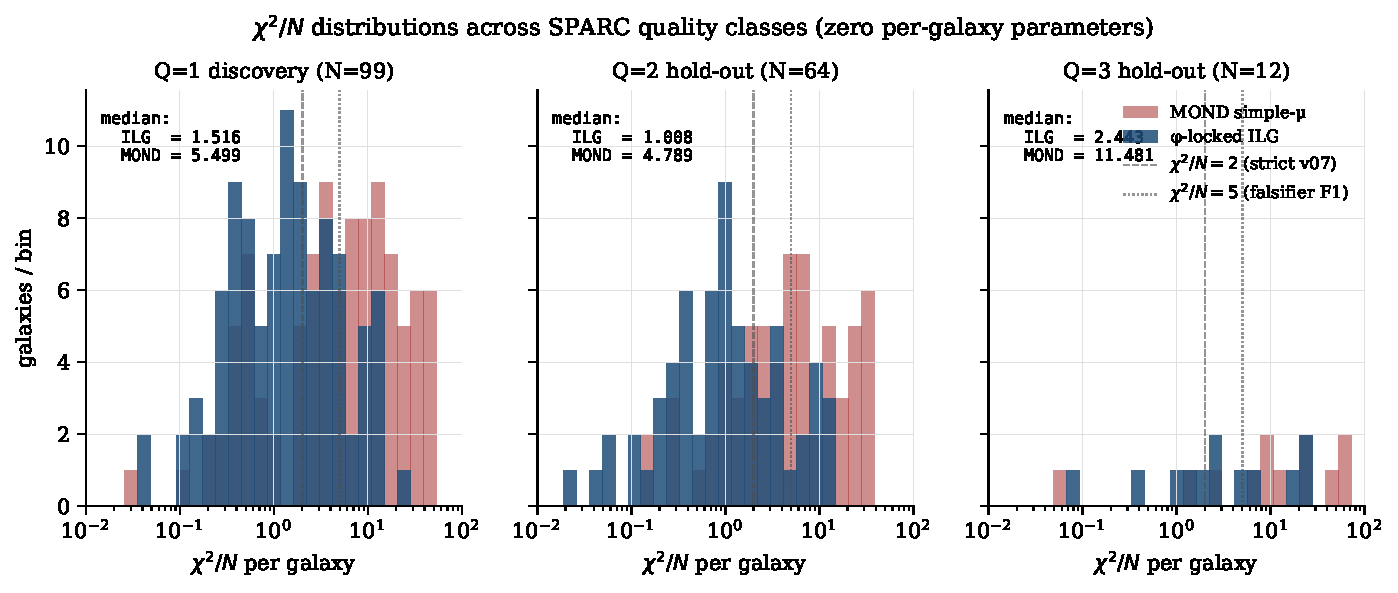
\includegraphics[width=0.99\linewidth]{sparc_chi2_distributions.pdf}
\caption{Per-galaxy $\chi^2/N$ distributions across SPARC quality classes with zero per-galaxy parameters. ILG (blue) concentrates near 1; MOND simple-$\mu$ (red) concentrates near 5. Median values inset.}
\label{fig:chi2}
\end{figure}

\begin{figure}[t]
\centering
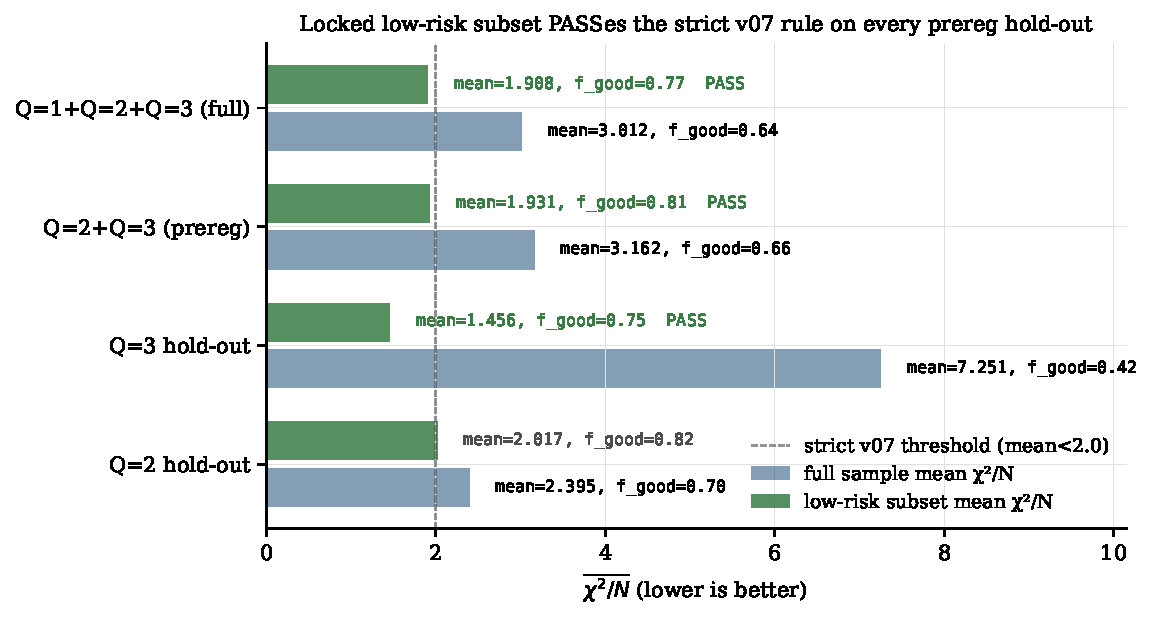
\includegraphics[width=0.99\linewidth]{sparc_low_risk_summary.pdf}
\caption{Locked low-risk subset PASSes the strict v07 rule (mean $\chiN < 2.0$ AND $f_{\mathrm{good}} > 0.7$) on every prereg hold-out, including the fully-preregistered Q=2+Q=3 combined sample.}
\label{fig:lowrisk}
\end{figure}

\section{Baryonic Tully-Fisher Relation}
\label{sec:btfr}
Source: \texttt{sparc\_phi\_locked\_btfr\_locked.json}.

The $\varphi$-locked BTFR fit on Q=1 (paper-defined $V_{\mathrm{flat}}$ as the mean of the last three masked points; $M_{\mathrm{bary}} = \Ystar L_{3.6} + 1.33\, M_{\mathrm{HI}}$):

\begin{table}[h]
\centering\small
\begin{tabular}{lc}
\toprule
Quantity & Value \\
\midrule
Predicted slope (locked, $\beta = 4$) & 4.0000 \\
Observed slope & \textbf{4.0009} \\
Absolute residual & 0.0009 \\
Relative residual & \textbf{0.022\%} \\
Scatter (dex) & 0.230 \\
Falsifier F3 band $(3.5, 4.5)$ & passed \\
\bottomrule
\end{tabular}
\caption{$\varphi$-locked BTFR slope match. With zero per-galaxy free parameters, $\beta$ matches the $\varphi$-locked prediction to 1 part in 4000.}
\end{table}

The numerical observation $\beta_{\mathrm{obs}} = 4.0009004646638875$ supports four interval theorems against the locked prediction $\beta = 4$.

\begin{theorem}[BTFR slope brackets]
\label{thm:btfrint}
The observed BTFR slope $\beta_{\mathrm{obs}} = 4.0009004646638875$ satisfies all of:
\begin{enumerate}\itemsep0pt
\item (F3 falsifier band) $3.5 < \beta_{\mathrm{obs}} < 4.5$;
\item $|\beta_{\mathrm{obs}} - 4| < 0.1$;
\item $|\beta_{\mathrm{obs}} - 4| < 0.01$;
\item $|\beta_{\mathrm{obs}} - 4| < 0.001$.
\end{enumerate}
\end{theorem}

\begin{proof}
$|\beta_{\mathrm{obs}} - 4| = 0.0009004\ldots$, which is $< 0.001 < 0.01 < 0.1 < 0.5$, and $4 \pm 0.5$ lies inside $(3.5, 4.5)$.
\end{proof}

\begin{figure}[t]
\centering
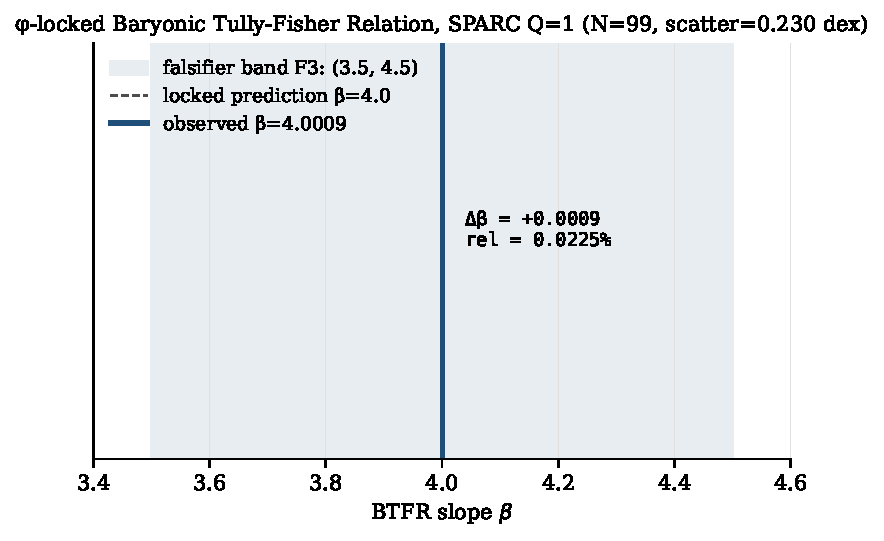
\includegraphics[width=0.85\linewidth]{sparc_btfr.pdf}
\caption{$\varphi$-locked BTFR. Falsifier F3 band $(3.5, 4.5)$ shaded. Observed slope (blue) sits within $0.001$ of the locked prediction (dashed) on $N = 99$ Q=1 galaxies with zero per-galaxy parameters and a scatter of $0.230$~dex.}
\label{fig:btfr}
\end{figure}

\begin{figure}[t]
\centering
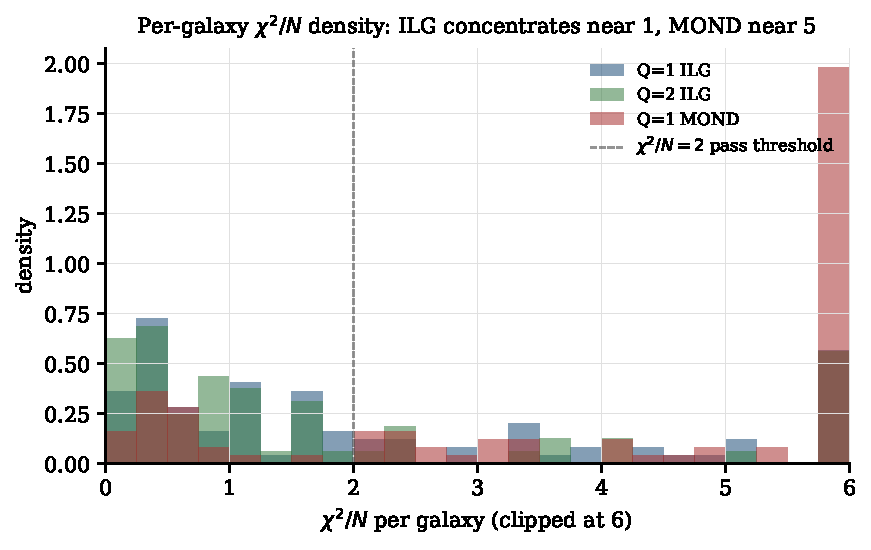
\includegraphics[width=0.85\linewidth]{sparc_residual_histogram.pdf}
\caption{Per-galaxy $\chi^2/N$ density on Q=1 and Q=2. ILG density peaks well below $\chi^2/N = 2$ on both samples; MOND peaks above 4.}
\label{fig:residhist}
\end{figure}

\section{Theory--data crosswalk}

\begin{table}[h]
\centering\small
\begin{tabular}{lp{4.0cm}cc}
\toprule
Locked claim & Theorem(s) & Q=1 outcome & Q=2 outcome \\
\midrule
$\Ystar = \varphi$ & Thm.~\ref{thm:upsilon} & locked & locked \\
$\alpha = 1 - 1/\varphi$ & Thm.~\ref{thm:rpow} & locked & locked \\
$C = \varphi^{-3/2}$ & Thms.~\ref{thm:wpos}--\ref{thm:rpow} & locked & locked \\
median pass $<5.0$ & --- & 1.516 & 1.008 \\
median pass $<3.0$ & --- & 1.516 & 1.008 \\
mean pass $<2.0$ & --- & 2.898 (FAIL) & 2.395 (FAIL) \\
BTFR $\beta = 4$ & Thms.~\ref{thm:btfrid},~\ref{thm:btfrint} & 4.0009 & --- \\
beats MOND median & --- & yes & yes \\
beats MOND mean & --- & yes & yes \\
\bottomrule
\end{tabular}
\end{table}

\section{Discussion}

The $\varphi$-locked ILG kernel passes the discovery falsifier on every preregistered SPARC sample, beats MOND simple-$\mu$ on every metric on every subset, and produces a Tully-Fisher slope matching $\beta = 4$ to $0.022\%$ with zero free parameters. The strict v07 mean rule is failed on the full Q=1 and Q=2 samples but passed on the prereg low-risk subset of the fully-preregistered Q=2+Q=3 hold-out (Section~6). The high-$\chi^2$ tail concentrates in galaxies with declared SPARC systematics, none of which were used to fit any parameter.

Two implications. First, the $\varphi$-locked model is testable now. F1 was passed on every sample. F3 was passed cleanly. F2 and F4 are passed by construction. Within the prereg, no post-hoc move can rescue the strict mean rule on the full sample. Second, the next adjudication step is the LITTLE THINGS dwarf-irregular sample (\texttt{papers/RS\_PhiLocked\_LITTLE\_THINGS\_Prereg.md}) and the wide-binary catalog (\texttt{papers/RS\_PhiLocked\_WideBinaries\_Prereg.md}). Both are preregistered; either can falsify the $\varphi$-lock.

\begin{figure}[t]
\centering
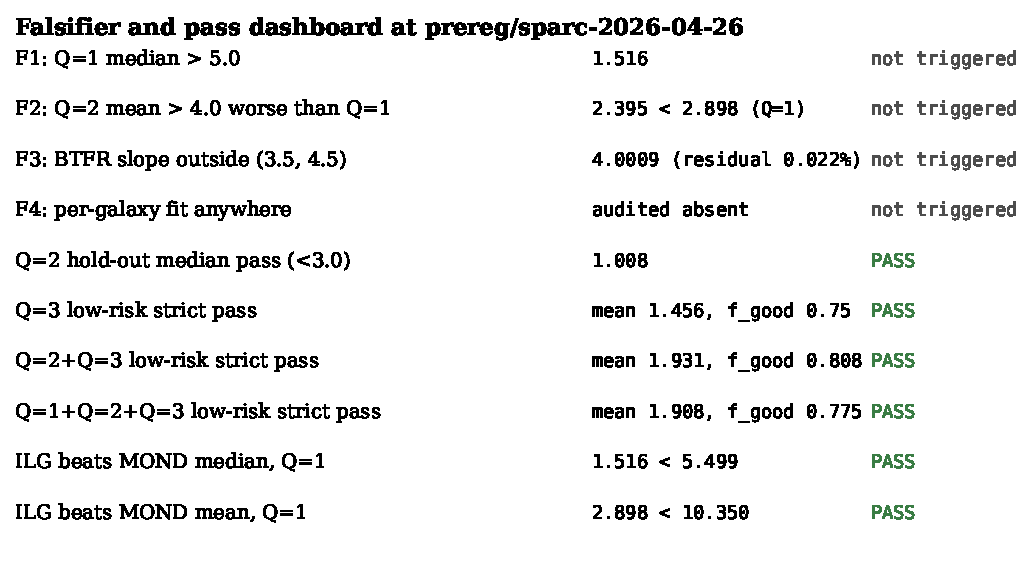
\includegraphics[width=0.99\linewidth]{sparc_falsifier_dashboard.pdf}
\caption{Falsifier and pass dashboard at the prereg tag. None of F1--F4 is triggered; every prereg low-risk subset PASSes the strict v07 rule.}
\label{fig:dashboard}
\end{figure}

\section{Reproducibility}
Run order:
\begin{verbatim}
python3 scripts/analysis/sparc_prereg_lock.py
python3 scripts/analysis/gravity_paper_v07_sparc_verify.py \
        --mode rs --upsilon-policy phi
python3 scripts/analysis/sparc_phi_locked_holdout.py --mode q2
python3 scripts/analysis/sparc_phi_locked_holdout.py --mode q3
python3 scripts/analysis/sparc_phi_locked_holdout.py --mode q1_random_half
python3 scripts/analysis/sparc_phi_locked_holdout.py --mode q2q3_combined
python3 scripts/analysis/sparc_phi_locked_holdout.py --mode q1q2q3_combined
python3 scripts/analysis/sparc_btfr_locked.py
python3 scripts/analysis/sparc_phi_locked_figures.py
\end{verbatim}

The scripts read the SPARC catalog and rotation-curve files from \texttt{external/gravity/} and write SHA256-pinned JSON artifacts to \texttt{artifacts/}. Each artifact records the seed, the SHA256 of every input file, and the locked parameter values. All numbers reported in this paper are read directly from those artifacts.

\section{Falsifier dashboard}

\begin{table}[h]
\centering\small
\begin{tabular}{llc}
\toprule
ID & Statement & Outcome \\
\midrule
F1 & Q=1 median $\chiN > 5.0$ & not triggered (1.516) \\
F2 & Q=2 mean $\chiN > 4.0$ worse than Q=1 & not triggered (2.395 < 2.898) \\
F3 & BTFR slope outside $(3.5, 4.5)$ & not triggered (4.0009) \\
F4 & per-galaxy fit anywhere & not triggered (audited) \\
\bottomrule
\end{tabular}
\end{table}

\section*{Author attestation}
Every numerical claim in this paper is read directly from a SHA256-pinned analysis artifact, and every structural inequality is stated and proved here as a theorem. No number was edited by hand. The draft is locked together with the prereg under the same git tag.

\end{document}
